\section{Controlling the Virtual Rover}

In \fig\ref{fig:acc_model} we depict the top-level model of the controller for
follower vehicle. The controller is meant to function in a loop by reading the
\emph{Velocity} of the follower rover itself, the velocity of the leader rover
(input by the \emph{VelocityFrontObstacle} signal) and the \emph{distance} to
the leader rover. By using these values it constantly updates the maximal
allowed acceleration (\emph{MaxAcceleration}) as well as
the target velocity (\emph{TargetVelocity}) for the follower rover.

The controller is composed by a number of \af components, as follows:
\begin{itemize}
  \item the \emph{TargetDistance} component is responsible for calculating the ideal
distance to the leader rover. This distance is proportional to the speed of
the leader, as larger speeds imply larger distances for breaking. 
  \item The \emph{P Controller} component is a PID controller for adjusting the
the velocity of the follower in order to reach the target distance to the
leader.
\item The \emph{TargetVelocityController} component decides whether the
\emph{TargetVelocity} output should remain the same as in the previous step
(saved in the \emph{MaxVelocityMemory}) or should be updated to the
\emph{TargetVelocityIn} calculated by the \emph{P Controller} component.
\levi{don't understand this part of the model}
\end{itemize}


\begin{figure}[!h]
\centering
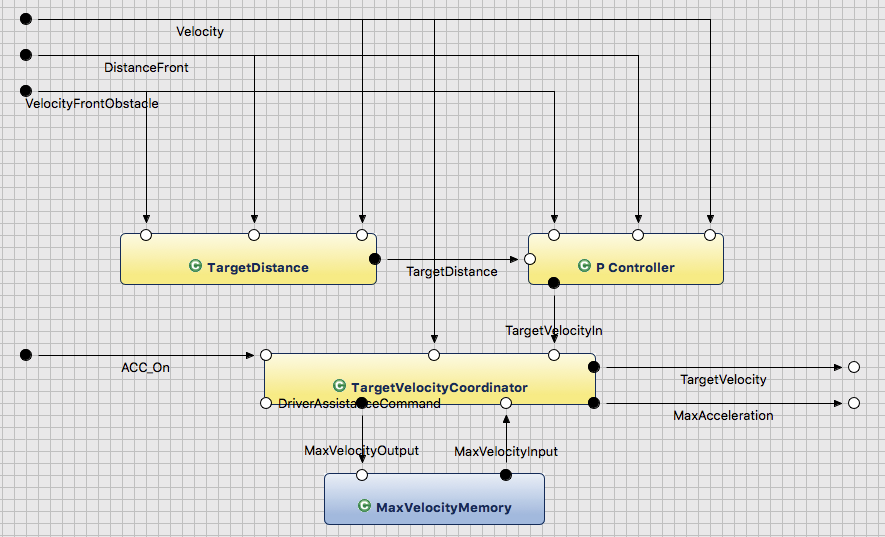
\includegraphics[width=1\textwidth]{images/ACC_controller_model.png}
\caption{The controller for the Automatic Cruise Control modelled in \af}
\label{fig:acc_model}
\end{figure}

\begin{figure}[!h]
\centering
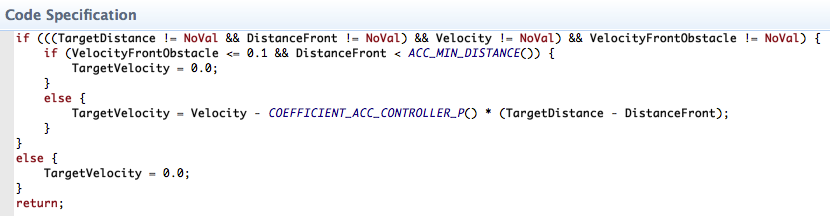
\includegraphics[width=1\textwidth]{images/code_spec_P_controller.png}
\caption{PID controller \af}
\label{fig:pid_controller}
\end{figure}

\begin{figure}[!h]
\centering
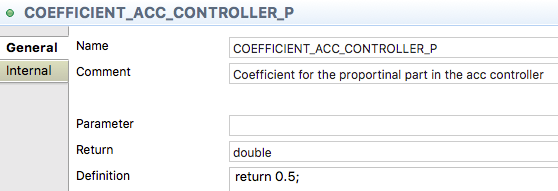
\includegraphics[width=.7\textwidth]{images/P_coefficient_controller.png}
\caption{P Coefficient}
\label{fig:p_coefficient}
\end{figure}